% Flowchart of the SORTIE algorithm. Compile with: pdflatex fig_algorithm.tex
\documentclass[border=4pt]{standalone}
\usepackage{amsmath,amssymb}
\usepackage{tikz}
\usetikzlibrary{arrows.meta,positioning,fit,backgrounds,calc,shapes.geometric}
\newcommand{\E}{\mathbb{E}}
\definecolor{cmain}{HTML}{2471A3}
\definecolor{cperturb}{HTML}{C0392B}
\definecolor{csupport}{HTML}{17A589}
\definecolor{cgrey}{HTML}{5D6D7E}
\begin{document}
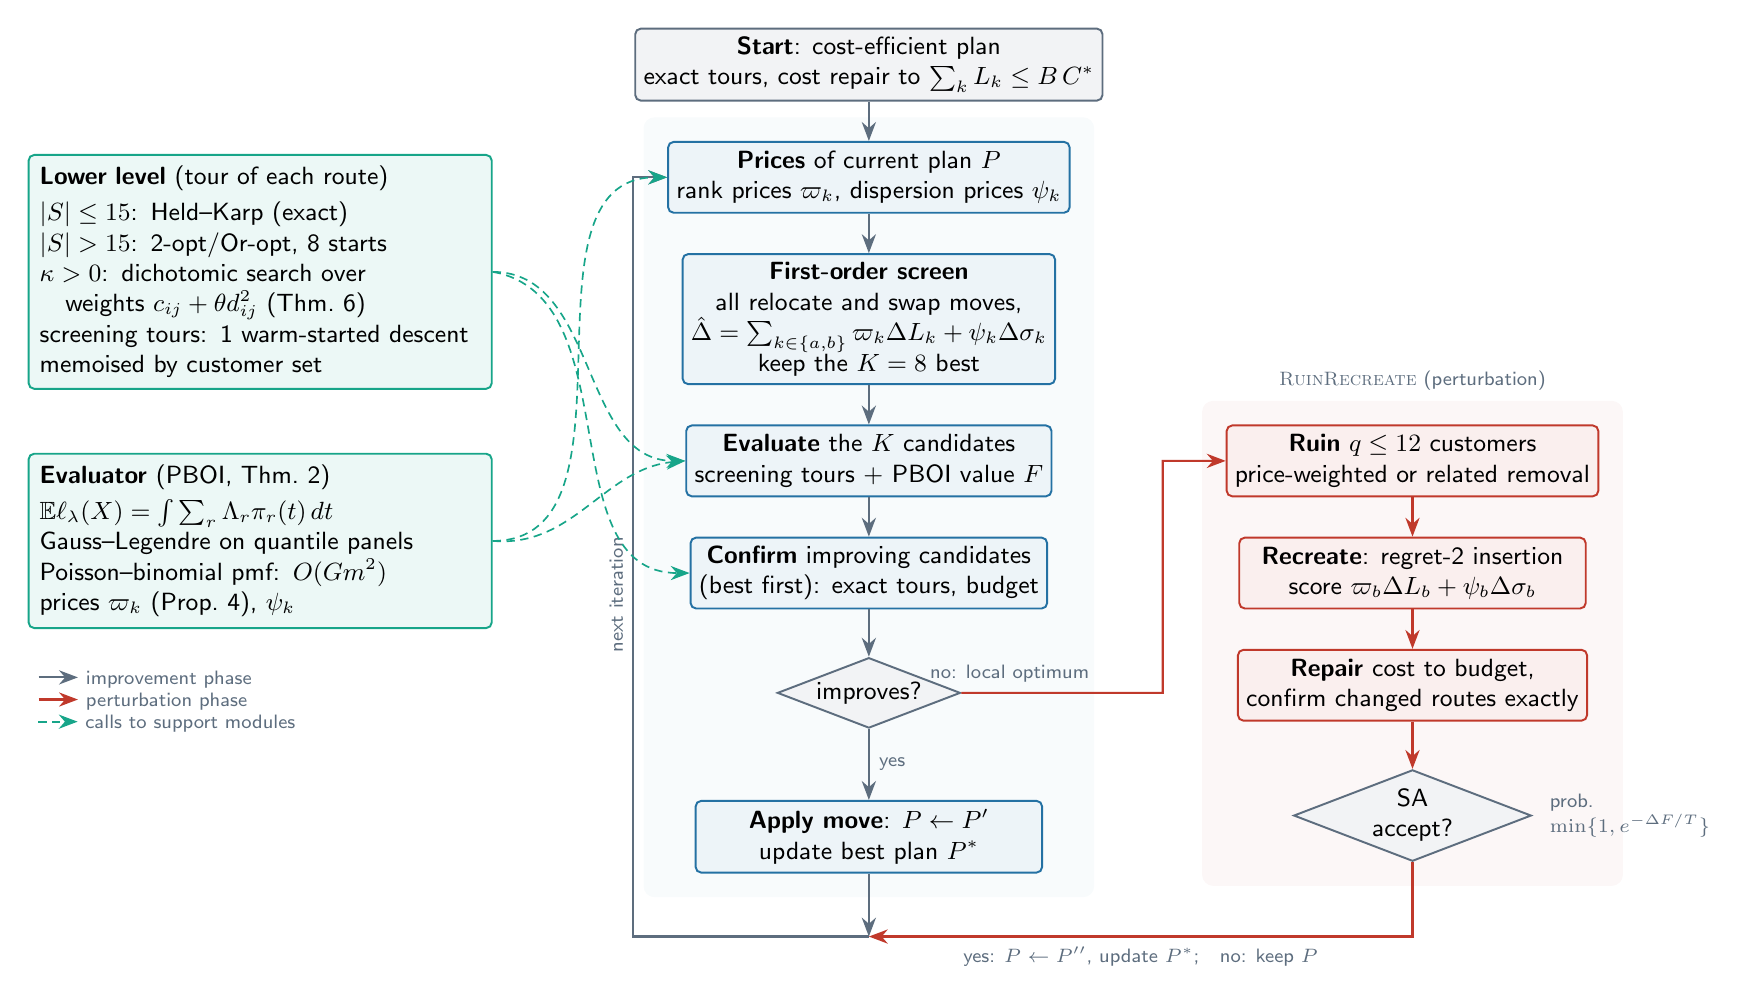
\begin{tikzpicture}[
  font=\sffamily\small,
  >={Stealth[length=2.4mm]},
  node distance=5mm and 9mm,
  box/.style={draw=#1, fill=#1!8, rounded corners=2pt, line width=0.7pt,
              align=center, minimum width=44mm, minimum height=9mm, inner sep=3pt},
  box/.default=cmain,
  dec/.style={draw=cgrey, fill=cgrey!8, diamond, aspect=2.6, align=center,
              inner sep=1pt, line width=0.7pt},
  sup/.style={draw=csupport, fill=csupport!8, rounded corners=2pt, line width=0.7pt,
              align=left, text width=56mm, inner sep=4pt},
  flow/.style={->, line width=0.8pt, draw=cgrey},
  call/.style={->, densely dashed, line width=0.6pt, draw=csupport},
  lab/.style={font=\sffamily\scriptsize, text=cgrey}
]

% ---------------- main column ----------------
\node[box=cgrey] (start) {\textbf{Start}: cost-efficient plan\\exact tours, cost repair to $\sum_k L_k\le B\,C^\ast$};
\node[box, below=of start] (prices) {\textbf{Prices} of current plan $P$\\rank prices $\varpi_k$, dispersion prices $\psi_k$};
\node[box, below=of prices] (screen) {\textbf{First-order screen}\\all relocate and swap moves,\\$\hat\Delta=\sum_{k\in\{a,b\}}\varpi_k\Delta L_k+\psi_k\Delta\sigma_k$\\keep the $K=8$ best};
\node[box, below=of screen] (evalK) {\textbf{Evaluate} the $K$ candidates\\screening tours $+$ PBOI value $F$};
\node[box, below=of evalK] (confirm) {\textbf{Confirm} improving candidates\\(best first): exact tours, budget};
\node[dec, below=6mm of confirm] (imp) {improves?};
\node[box, below=9mm of imp] (accept) {\textbf{Apply move}: $P\gets P'$\\update best plan $P^\ast$};

% ---------------- perturbation column ----------------
\node[box=cperturb, right=22mm of evalK] (ruin) {\textbf{Ruin} $q\le 12$ customers\\price-weighted or related removal};
\node[box=cperturb, below=of ruin] (recreate) {\textbf{Recreate}: regret-2 insertion\\score $\varpi_b\Delta L_b+\psi_b\Delta\sigma_b$};
\node[box=cperturb, below=of recreate] (repair) {\textbf{Repair} cost to budget,\\confirm changed routes exactly};
\node[dec, below=6mm of repair] (sa) {SA\\accept?};
\node[lab, right=1mm of sa, align=left] {prob.\\$\min\{1,e^{-\Delta F/T}\}$};

% ---------------- support modules ----------------
\node[sup, left=24mm of screen, yshift=6mm] (lower) {\textbf{Lower level} (tour of each route)\\[2pt]
  $|S|\le15$: Held--Karp (exact)\\
  $|S|>15$: 2-opt/Or-opt, 8 starts\\
  $\kappa>0$: dichotomic search over\\\quad weights $c_{ij}+\theta d_{ij}^2$ (Thm.~6)\\
  screening tours: 1 warm-started descent\\
  memoised by customer set};
\node[sup, below=8mm of lower] (pboi) {\textbf{Evaluator} (PBOI, Thm.~2)\\[2pt]
  $\E\ell_\lambda(X)=\int\sum_r\Lambda_r\pi_r(t)\,dt$\\
  Gauss--Legendre on quantile panels\\
  Poisson--binomial pmf: $O(Gm^2)$\\
  prices $\varpi_k$ (Prop.~4), $\psi_k$};

% ---------------- main flow ----------------
\draw[flow] (start) -- (prices);
\draw[flow] (prices) -- (screen);
\draw[flow] (screen) -- (evalK);
\draw[flow] (evalK) -- (confirm);
\draw[flow] (confirm) -- (imp);
\draw[flow] (imp) -- node[lab, right] {yes} (accept);
\coordinate[below=8mm of accept] (J);
\draw[flow] (accept) -- (J);
\draw[flow] (J) -- ++(-30mm,0) coordinate (Jl) |- (prices.west);
\node[lab, rotate=90, anchor=south] at ($(Jl)!0.45!(Jl|-prices.west)$) {next iteration};

% no improving move -> perturbation
\draw[flow, draw=cperturb] (imp.east) -| node[lab, pos=0.12, above] {no: local optimum} ($(ruin.south west)!0.5!(ruin.north west)+(-8mm,0)$) -- (ruin.west);
\draw[flow, draw=cperturb] (ruin) -- (recreate);
\draw[flow, draw=cperturb] (recreate) -- (repair);
\draw[flow, draw=cperturb] (repair) -- (sa);
\draw[flow, draw=cperturb] (sa.south) |- node[lab, pos=0.75, below, align=center] {yes: $P\gets P''$, update $P^\ast$;\quad no: keep $P$} (J);

% ---------------- support calls ----------------
\draw[call] (lower.east) to[out=0, in=180] (evalK.west);
\draw[call] (lower.east) to[out=-10, in=180] (confirm.west);
\draw[call] (pboi.east) to[out=0, in=180] (prices.west);
\draw[call] (pboi.east) to[out=-5, in=185] (evalK.west);

% ---------------- legend ----------------
\node[lab, align=left, anchor=north west] at ($(pboi.south west)+(0,-4mm)$)
  {\tikz\draw[flow] (0,0)--(5mm,0); improvement phase\\
   \tikz\draw[flow,draw=cperturb] (0,0)--(5mm,0); perturbation phase\\
   \tikz\draw[call] (0,0)--(5mm,0); calls to support modules};

% ---------------- phase backgrounds ----------------
\begin{scope}[on background layer]
  \node[fill=cmain!3, rounded corners=4pt, inner sep=3mm,
        fit=(prices)(screen)(evalK)(confirm)(imp)(accept)] {};
  \node[fill=cperturb!4, rounded corners=4pt, inner sep=3mm,
        fit=(ruin)(recreate)(repair)(sa),
        label={[lab, anchor=south]north:{\textsc{RuinRecreate} (perturbation)}}] {};
\end{scope}
\end{tikzpicture}
\end{document}
